\documentclass[10pt,twocolumn,letterpaper]{article}

\usepackage{cvpr}
\usepackage{times}
\usepackage{epsfig}
\usepackage{graphicx}
\usepackage{amsmath}
\usepackage{amssymb}

\usepackage{subfigure}
\usepackage{algorithm}
\usepackage{algorithmic}
\usepackage{mathrsfs}
\usepackage{soul}
\usepackage{multirow}
\usepackage{comment}
\usepackage{tabularx}
\usepackage[tableposition=top]{caption}
\usepackage{pbox}

%\usepackage[sort&compress,square,comma]{natbib}

\usepackage{pgfplots}
\usepackage{pgfplotstable}
\usepackage{filecontents,pgfplots}
\usepackage{tikz}
\usetikzlibrary{shapes,matrix,arrows,decorations.pathmorphing, positioning, calc, decorations.markings}
\usepackage{sci}
\renewcommand{\algorithmicrequire}{\textbf{Input:}}
\renewcommand{\algorithmicensure}{\textbf{Output:}}


% Include other packages here, before hyperref.
\usepackage{stackengine}

% If you comment hyperref and then uncomment it, you should delete
% egpaper.aux before re-running latex.  (Or just hit 'q' on the first latex
% run, let it finish, and you should be clear).
\usepackage[pagebackref=true,breaklinks=true,letterpaper=true,colorlinks,bookmarks=false]{hyperref}

\cvprfinalcopy % *** Uncomment this line for the final submission

\def\cvprPaperID{725} % *** Enter the CVPR Paper ID here
\def\httilde{\mbox{\tt\raisebox{-.5ex}{\symbol{126}}}}

% Pages are numbered in submission mode, and unnumbered in camera-ready
\ifcvprfinal\pagestyle{empty}\fi
\begin{document}

%%%%%%%%% TITLE
\title{Deep Relative Attributes}

\author{Yaser Souri$^1$, Erfan Noury$^2$, Ehsan Adeli-Mosabbeb$^3$\\
$^1$Sobhe \quad $^2$Sharif University of Technology \quad $^3$University of North Carolina at Chapel Hill\\
{\tt\small souri@sobhe.ir, erfan.noury@live.com, eadeli@unc.edu}
%\and
%Erfan Noury\\
%Sharif University of Technology\\
%{\tt\small noury@ce.sharif.edu}
%\and
%Ehsan Adeli Mosabbeb\\
%University of North Carolina at Chapel Hill\\
%{\tt\small eadeli@unc.edu}
}

\maketitle
%\thispagestyle{empty}

%%%%%%%%% ABSTRACT
\begin{abstract}
Visual attributes are great means of describing images or scenes, in a way both humans and computers understand. In order to establish a correspondence between images and to be able to compare the strength of each property between images, relative attributes were introduced. However, since their introduction, hand-crafted and engineered features were used to learn complex models for the problem of relative attributes. This limits the applicability of those methods for more realistic cases. We introduce a two part deep learning architecture for the task of relative attribute prediction. A convolutional neural network (ConvNet) architecture is adopted to learn the features with addition of an additional layer (ranking layer) that learns to rank the images based on these features. Also an appropriate ranking loss is adapted to train the whole network in an end-to-end fashion. Our proposed method outperforms the baseline and state-of-the-art methods in relative attribute prediction on various datasets. Our qualitative results also show that the network is able to learn effective features for the task. Furthermore, we use our trained models to visualize saliency maps for each attribute.
\end{abstract}



% !TeX root=arxiv.tex
% !TEX TS-program = pdfLatex

%%%%%%%%%%%%%%%%%%%%%% INTRODUCTION %%%%%%%%%%%%%%%%%%%%%%%%%%%%%%
\section{Introduction}

%  After the "Relative Attributes" paper \cite{parikh2011}, there was a stream of papers that aimed to solve the same or similar task (\cite{Li2013,Yu2014,Sandeep_2014_CVPR,Lee_2013_7540}) using a different and often more complex model instead of the original RankSVM model. I think as progress in the "Visual Recognition" field has shown, for solving the problem you actually need to change the features not the model. So in this project I actually want to experiment with how learning the features end-to-end (or fine-tuning the features) can improve Relative Attributes accuracy and power. 
 
%  Please follow the notations as in here\footnote{\notation}. We will remove this footnote. I just put it here, so that we all know how to write the formulations. Use \



Visual attributes are linguistic terms that bear semantic properties of (visual) entities, often shared among categories. They are both human understandable and machine detectable, which makes them appropriate for better human machine communications. Visual attributes have been successfully used for many applications, such as image search \cite{whittlesearch}, interactive fine-grained recognition \cite{branson13, branson10} and zero-shot learning \cite{6571196, parikh2011}.

Traditionally, visual attributes were treated as binary concepts \cite{ferrari2007learning, Farhadi09describingobjects}, as if they are present or not, in an image.
% or a scene.
Parikh and Grauman ~\cite{parikh2011} introduced a more natural view on visual attributes, in which pairs of visual entities can be compared, with respect to their relative strength of any specific property. With a set of human assessed relative orderings of image pairs, they learn a global ranking function for each attribute (Figure \ref{fig.1}).
While binary visual attributes relate properties to entities (\eg, a dog being furry), relative attributes makes it possible to relate entities to each other in terms of their properties (\eg, a bunny being furrier than a dog).

\begin{figure}
\centering
\scalebox{.3}
{
\begin{tikzpicture}
	% pair 1
	\node (p1A) {
\includegraphics[scale=0.65]{Fig1/pair1A.jpg}};
	\node (p1op) [right=0.0cm of p1A, scale=3] {$>$};
	\node (p1B) [right=-0.4cm of p1op] {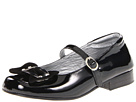
\includegraphics[scale=0.65]{Fig1/pair1B.jpg}};

	\draw[line width=2, rounded corners] ($(p1A.north west)+(-0.0,0.5)$)  rectangle ($(p1B.south east)+(0.0,-0.5)$);
	
	% pair 2
	\node (p2B) [right=0.0cm of p1B] {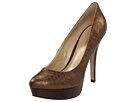
\includegraphics[scale=0.65] {Fig1/pair2B.jpg}};
	\node (p2op) [right=0.0cm of p2B, scale=3] {$<$};
	\node (p2A) [right=-0.4cm of p2op] {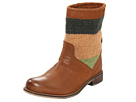
\includegraphics[scale=0.65] {Fig1/pair2A.jpg}};

	\draw[line width=2, rounded corners] ($(p2B.north west)+(0.2,0.5)$) rectangle ($(p2A.south east)+(0.0, -0.5)$);

	% dots
	\node (dots) [right=0.1cm of p2A, scale=4] {\dots};

	% pair3
	\node (p3A) [right=0.0cm of dots] {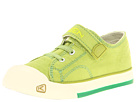
\includegraphics[scale=0.65]{Fig1/pair3A.jpg}};
	\node (p3op) [right=0.0cm of p3A, scale=3] {$>$};
	\node (p3B) [right=-0.4cm of p3op] {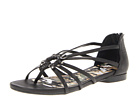
\includegraphics[scale=0.65]{Fig1/pair3B.jpg}};

	\draw[line width=2, rounded corners] ($(p3A.north west)+(-0.2,0.5)$) rectangle ($(p3B.south east)+(0.2, -0.5)$);

	% Training phase box and label	
% 	\draw[line width=2, rounded corners, red, loosely dotted] ($(p1A.north west)+(-0.4, 1)$) rectangle ($(p3B.south east)+(0.4, -1)$);

% 	\path (p1A.north east) -- (p3B.north west) node [scale=3, above=1cm, pos=0.5] {Training};

	% bottom mid point
	\path (p1A.south east) -- (p3B.south west) node (mid) [below=1cm, pos=0.5] {};

	% testing pair
	\node (uop) [below=4cm of mid, scale=4] {$?$};
	\node (puA) [left=0.5cm of uop] {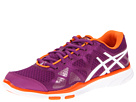
\includegraphics[scale=1]{Fig1/pairUA.jpg}};
	\node (puB) [right=0.5cm of uop] {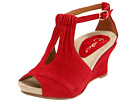
\includegraphics[scale=1]{Fig1/pairUB.jpg}};
	
	\draw [line width=2, rounded corners, dashed] ($(puA.north west)+(-0.2, 0.5)$) rectangle ($(puB.south east)+(0.2, -0.5)$);
	
	% testing phase arrow
	\path [draw, ->, line width=10] (mid.south) -- ($(uop.north) + (0cm, 2cm)$);	

\end{tikzpicture}}
\caption{Visual Relative Attributes. This figure shows samples of training pairs of images from the UT-Zap50K dataset, comparing shoes in terms of `comfort' (top). The goal is to compare a pair of two novel shoe images, respective to the same attribute (bottom).}
\label{fig.1}
\end{figure}

Many have tried to build on the seminal work of Parikh and Grauman \cite{parikh2011} with more complex and task specific models for ranking, while still using hand crafted visual features, such as GIST \cite{Aude01} and HOG \cite{hog}. Recently, Convolutional Neural Networks (ConvNets) have proved to be successful in various visual recognition tasks, such as image classification \cite{krizshevsky}, object detection \cite{RCNN} and image segmentation \cite{fullyconv}. Many attribute the success of ConvNets to their ability to learn multiple layers of visual features from data. 

In this work, we propose to use a ConvNet-based architecture to learn the ranking of images, using relatively annotated images for each attribute. Pairs of images with similar and/or different strengths of some particular attribute are presented to the network. The network  learns a series of visual features, which are known to work better than engineered visual features \cite{offtheshelf}. After learning the features, we further propose to add another layer to the network, to rank the images. The ranking layer could be learned through gradient descent (described in more details later). As a result, it would be possible to learn (or fine-tune) the features through back-propagation, while learning the ranking layer. Interweaving the two processes leads to a set of learned features that characterize each single attribute. This escalates the overall performance and is the main advantage of our proposed method over previous methods. Furthermore, in almost all previous works on relative attributes, the training phase often can only handle inequality relations (\ie, one image being less or more strong, in terms of a specific attribute, than the other). The equality relation can happen quite frequently when humans are qualitatively deciding about the relations of attributes in images. In previous works this is not explored, even in some, the equality relation could not be incorporated in the training phase, due to method limitations. Our proposed method introduces an easy and elegant way to deal with equality relations (\ie, an attribute is similarly strong in two images).
%%%%%%%%%%%% spatial extent shall be removed from the paper
%It is noteworthy to pinpoint that by exploiting the saliency maps of the unsupervised learned features for each attribute, similar to \cite{simonyan14a}, we can discover the spatial extent \cite{specialextent} of the attribute. %This is done using the same network in an unsupervised manner.
%%%%%%%%%%%% spatial extent shall be removed from the paper

Our approach achieves very competitive results and improves the state-of-the-art (with a large margin in some datasets) on major publicly available datasets for relative attributes, both coarse-grained and fine-grained.

% (we might need to save some space.) No need for this:  (If we had extra space, we can put it back... )
The rest of the paper is organized as follows: Section \ref{sec.2} discusses the related works. Section \ref{sec.3} illustrates our proposed method, including the ConvNet for learning the feautres and the ranking layer. Then, Section \ref{sec.4} exhibits the experimental setup and results, and finally, Section \ref{sec.5} concludes the paper.


% !TeX root=arXiv.tex
% !TEX TS-program = pdfLatex

%%%%%%%%%%%%%%%%%%%%%%%%%% RELATED WORKS %%%%%%%%%%%%%%%%%%%%%%%%%
\section{Related Works}
\label{sec.2}

We usually describe visual concepts with their attributes, and how they look. Attributes are, therefore, mid-level representations for describing objects and scenes. In an early work on attributes, Farhadi \etal~\cite{Farhadi09describingobjects} proposed to describe objects using mid-level attributes. In another work \cite{farhadi10}, they described images based on their attributes, basically a semantic triple <object, action, scene>. Later, Han \etal~\cite{6739133} proposed to describe images at different semantic levels. In the recent years, attributes have shown great performance in object recognition \cite{Farhadi09describingobjects,7298613}, action recognition \cite{6838985,5995353} and event detection \cite{6475038}. Lampert \etal~\cite{6571196} predicted unseen objects using a zero-shot learning framework, in which binary attribute representation of the objects were incorporated. 

On the other hand, comparing attributes enables us to easily and reliably search through high-level data derived from \eg, documents or images. For instance, Kovashka \etal~\cite{KovashkaG13} proposed a relevance feedback strategy for image search using attributes and their comparisons. In order to establish the capacity for comparing attributes, we need to move from binary attributes towards describing attributes relatively. In the recent years, relative attributes have attracted the attention of many researchers, in which a global function is learned for each single attribute. For instance, a linear relative comparison function is learned in \cite{parikh2011}, based on RankSVM \cite{Joachims2002} and a non-linear strategy in \cite{Li2013}. In another work, Datta \etal~\cite{5771429} used trained rankers for each facial image feature and formed a global ranking function for attributes.

Through the process of learning the attributes, different types of low-level image features are incorporated. For instance, Parikh and Grauman~\cite{parikh2011} used 512-dimensional GIST \cite{Aude01} descriptors as image features, while Jayaraman \etal\cite{6909607} used histograms of image features, and reduced their dimensionality using PCA. Other works tried learning attributes through \eg, local and learning \cite{1641014} or fine-grained comparisons \cite{Yu2014}. Yu and Grauman \cite{Yu2014} proposed a local learning-to-rank framework for fine-grained visual comparisons, in which the ranking model is learned using only analogous training comparisons. In another work \cite{Yu2015}, they proposed a local bayesian model to rank images, which are indistinguishable for a given attribute. 

As could be inferred from the literature, it is very hard to decide what low-level image features to use for identifying and comparing visual attributes. Recent studies show that features learned through the convolutional neural networks (CNNs) \cite{NIPS1989_293} (also known as deep features) could achieve great performance for image-based recognition \cite{NIPS2012_4824} and object detection \cite{6909475}. Zhang \etal~\cite{6909608} utilized CNNs for classifying binary attributes. In other works, Escorcia \etal~\cite{Escorcia_2015_CVPR} proposed CCNs with attribute centric nodes within the net for establishing the relationships between visual attributes, Shankar \etal~\cite{Shankar_2015_CVPR} proposed a weakly supervised setting on convolutional neural networks, applied for attribute detection, and Khan \etal~\cite{khan15} used deep features for describing human attributes and thereafter for action recognition. 

CNNs and neural networks have also been extended for learning-to-rank applications. One of the earliest networks for ranking was proposed by Burges\etal~\cite{Burges2005}, known as RankNet. The underlying model in RankNet maps an input feature vector to a Real number. The model is trained  by presenting the network with pairs of input training feature vectors with differing labels. Then based on how they should have been ranked, the underlying model parameters are updated. This model has been used in different fields for ranking and retrieval applications, \eg, for personalized search \cite{song2014} or content-based image retrieval \cite{Wan2014}. 



% !TeX root=arXiv.tex
% !TEX TS-program = pdfLatex

%%%%%%%%%%%%%%%%%%%%%%% END-TO-END DEEP RELATIVE ATTRIBUTES %%%%%%%%%%%%%%%
\section{Proposed Method}
\label{sec.3}

We propose to use a ConvNet-based deep neural network that is trained to optimize an appropriate ranking loss for the task of predicting relative attribute strength. The network architecture consists of two parts, the \textit{feature learning and extraction} part and the \textit{ranking} part.

The feature learning and extraction part takes a fixed size image, $I_i$, as input and outputs the learned feature representation for that image $\psi_i \in \mathbb{R}^d$.
%Different network architectures have been developed in the literature over the past few years, for extracting and learning features in a deep framework that almost all of them are applicable. 
Over the past few years, different network architectures for computer vision problems have been developed. These deep architectures can be used for extracting and learning features for different applications.
For the current work, outputs of an intermediate layer, like the last layer before the probability layer, from a ConvNet architecture (\eg, AlexNet \cite{krizshevsky}, VGGNet \cite{verydeep} or GoogLeNet \cite{googlenet}) can be incorporated. %used.

One of the most widely used models for relative attributes in the literature is RankSVM \cite{Joachims2002}. However,
%here, we want a neural network based ranking procedure that accepts relatively ordered pairs of feature vectors as input during training,
in our case, we seek a neural network based ranking procedure, to which relatively ordered pairs of feature vectors are inputted during training. This procedure should learn to map each feature vector to an absolute ranking, for testing purpose. Burges \etal~\cite{Burges2005} introduced such a neural network based ranking procedure that exquisitely fits our needs. %with our desired properties. The ranking part of our proposed network architecture is thus similar (reffered to as RankNet).
We adopt a similar strategy and thus, the ranking part of our proposed network architecture is analogous to \cite{Burges2005} (referred to as RankNet).

During training for a minibatch of image pairs and their target orderings, the output of the feature learning and extraction part of the network is fed into the ranking part and a ranking loss is computed. The loss is then back-propagated through the network, which enables us to simultaneously learn the weights of both feature learning and extraction (ConvNet) and ranking (RankNet) parts of the network. %Further, with simple techniques 
Further with back-propagation we can calculate the derivative of the estimated ordering with respect to the pixel values.
In this way, we can simply generate saliency maps for each attribute (see section \ref{sec.4.5}). These saliency maps exhibit interesting properties, as they can be used to localize the pixels in the image that are informative about the strength of presence of the attribute.

\subsection{RankNet: Learning to Rank Using Gradient Descent}\label{sec3.1}

This section briefly overviews the RankNet \cite{Burges2005} procedure in our context.
Given a set of pairs of sample feature vectors $\big\{( \psi_{1}^{(k)}, \psi_{2}^{(k)} ) | k \in \{1, \dots, n\} \big\} \in \mathbb{R}^{d \times d}$, and target probabilities $\big\{ t_{12}^{(k)} | k \in \{1, \dots, n\} \big\}$, % that 
sample $\psi_{1}^{(k)}$ is to be ranked higher than sample $\psi_{2}^{(k)}$. %, we want 
We would like to learn a ranking function $f : \mathbb{R}^d \mapsto \mathbb{R}$, such that $f$ specifies the ranking order of a set of features. Here, $f(\psi_i) > f(\psi_j)$ indicates that the %model thinks that 
feature vector $\psi_i$ is ranked higher than $\psi_j$, denoted by $\psi_i \triangleright \psi_j$. The RankNet model \cite{Burges2005} provides an elegant procedure based on neural networks %based way
to learn the function $f$.

Denoting $r_i \equiv f(\psi_i)$, RankNet models the mapping from rank estimates to posterior probabilities $p_{ij} = P(\psi_i \triangleright \psi_j)$ using a logistic function 

\begin{equation}
p_{ij} := \frac{1}{1 + e^{-(r_i - r_j)}}.
\end{equation}

The loss for the sample pair of feature vectors $(\psi_i, \psi_j)$ along with target probability $t_{ij}$ is defined as

\begin{equation}
C_{ij} := - t_{ij} \log (p_{ij}) - (1 - t_{ij}) \log (1 - p_{ij}),
\end{equation}

which is the binary cross entropy loss.
Figure \ref{fig.2} (left) plots the loss value $C_{ij}$ as a function of $r_i - r_j$ for three values of target probability $t_{ij} \in \{0, 0.5, 1\}$. This function is quite suitable for ranking purposes, as it acts differently compared to regression functions.

Specifically, we are not interested in regression instead of the ranking for two reasons: First, we cannot regress the absolute rank of images, since the annotations are only available in pairwise ordering for each attribute, in relative attribute datasets (see section \ref{sec.4.1}). Second, regressing the difference $r_i - r_j$ to $t_{ij}$ is also inappropriate.
Let's consider the squared loss

\begin{equation}
R_{ij} = \big[(r_i - r_j) - t_{ij}\big]^2,
\end{equation}

which is typically used for regression, illustrated in Figure \ref{fig.2} (right). We observe that the regression loss forces the difference of rank estimates to be a specific value and disallows over-estimation. Furthermore, its quadratic natures makes it %very
sensitive to noise. This sheds light into why regression objective is the wrong objective to optimize when the goal is ranking.

\begin{figure}
    \centering
    \begin{subfigure}
        \centering
        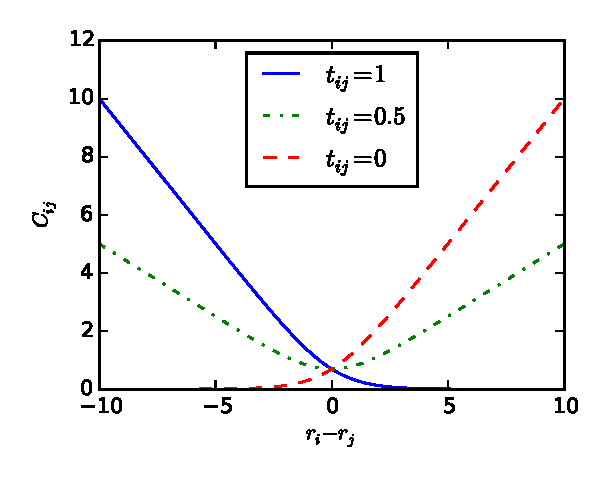
\includegraphics[width=4cm]{fig2-2/fig3.eps}
    \end{subfigure}
    \begin{subfigure}
        \centering
        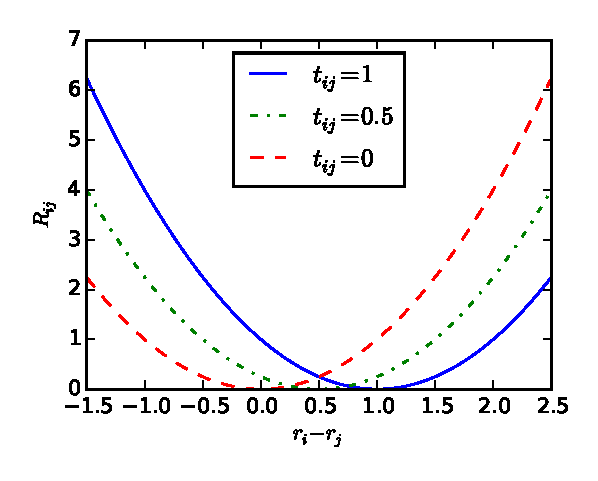
\includegraphics[width=4cm]{fig2-2/fig3-reg.eps}
    \end{subfigure}
    \caption{The ranking loss value for three values of the target probability (left). The squared loss value for three values of the target probability, typically used for regression (right).}
    \label{fig.2}
\end{figure}

Note that when $t_{ij} = 0.5$, and no information is available about the relative rank of the two samples, the ranking cost becomes symmetric. This can be used as a way to train on patterns that are desired to have similar ranks. This is somewhat scarce in the previous works on relative attributes.
Furthermore, this model asymptotically converges to a linear function which makes it more appropriate for problems with noisy labels. %than quadratic loss functions.

Training this model is possible using stochastic gradient descent or its variants like RMSProp.%, which is also used in our proposed method.
While testing, we only need to estimate the value of $f(\psi_i)$, which resembles the absolute rank of the test sample. Using $f(\psi_i)$s, we can easily infer the relative ordering or absolute ordering of test pairs.

\subsection{Deep Relative Attributes}\label{sec3.2}

%%%%%%%%%%%%%%%%%%%%%%%% Figure 3 %%%%%%%%%%%%%%%%%%%%%%%%%%%%%%%%%%%%%%%%%%%%%%%%%%%%%
\begin{figure*}
\centering
\scalebox{.3}
{
% We need layers to draw the block diagram
\pgfdeclarelayer{background}
\pgfdeclarelayer{foreground}
\pgfsetlayers{background,main,foreground}

% Define a few styles and constants
\tikzstyle{sensor}=[draw, fill=blue!20, text width=5em, 
    text centered, minimum height=2.5em]
\tikzstyle{ann} = [above, text width=5em]
\tikzstyle{naveqs} = [sensor, text width=6em, fill=red!20, 
    minimum height=12em, rounded corners]
\def\blockdist{2.3}
\def\edgedist{2.5}

\begin{tikzpicture}
    % feature extraction part rectangle
	% images
	\node (im1) at (0cm,1cm) [draw] {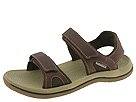
\includegraphics[scale=1]{Fig2/im1.jpg}};
	\node (im2) at (0cm, -6cm) [draw] {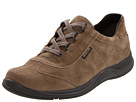
\includegraphics[scale=1]{Fig2/im2.jpg}};

	% topconv1 layer
	\node (tconv1) at (5.1cm, 1cm) {};
%	\draw [fill=blue!20] (5.6cm,3.1cm) rectangle (9.6cm,0.1cm);
	\draw [fill=blue!20] (5.4cm,2.9cm) rectangle (9.4cm,-0.1cm);
	\draw [fill=blue!20] (5.2cm,2.7cm) rectangle (9.2cm,-0.3cm);
	\draw [fill=blue!20] (5cm,2.5cm) rectangle (9cm,-0.5cm);

	% bottomconv1 layer
	\node (bconv1) at (5.1cm, -6cm) {};
%	\draw [fill=blue!20] (5.6cm,-3.9cm) rectangle (9.6cm,-6.9cm);
	\draw [fill=blue!20] (5.4cm,-4.1cm) rectangle (9.4cm,-7.1cm);
	\draw [fill=blue!20] (5.2cm,-4.3cm) rectangle (9.2cm,-7.3cm);
	\draw [fill=blue!20] (5cm,-4.5cm) rectangle (9cm,-7.5cm);

	% arrows from images to conv1s
	\path [draw, ->, line width=3] (im1.east) -- node [above, scale=3] {$I_i$} (tconv1);
	\path [draw, ->, line width=3] (im2.east) -- node [above, scale=3] {$I_j$} (bconv1);

	% topconv2 layer
	\node (tconv2) at (12cm, 1cm) {};
	\draw [fill=blue!20] (12.6cm,3.1cm) rectangle (16.6cm,0.1cm);
	\draw [fill=blue!20] (12.4cm,2.9cm) rectangle (16.4cm,-0.1cm);
	\draw [fill=blue!20] (12.2cm,2.7cm) rectangle (16.2cm,-0.3cm);
	\draw [fill=blue!20] (12cm,2.5cm) rectangle (16cm,-0.5cm);

	% bottomconv2 layer
	\node (bconv2) at (12cm, -6cm) {};
	\draw [fill=blue!20] (12.6cm,-3.9cm) rectangle (16.6cm,-6.9cm);
	\draw [fill=blue!20] (12.4cm,-4.1cm) rectangle (16.4cm,-7.1cm);
	\draw [fill=blue!20] (12.2cm,-4.3cm) rectangle (16.2cm,-7.3cm);
	\draw [fill=blue!20] (12cm,-4.5cm) rectangle (16cm,-7.5cm);

	\path (tconv1.east)+(4.65cm, 0cm) -- node [scale=4]{\dots} (tconv2);
	\path (bconv1.east)+(4.65cm, 0cm) --node [scale=4]{\dots} (bconv2);

	\node (convnet) [below, scale=3.5] at (11cm, -8cm) {ConvNet};

	% toprank
	\node (tconvout) at (16.6cm, 1cm) {};
	\node (trank) at (21.1cm, 1cm) [rectangle, draw, fill=red!20, scale=3, align=center] {Ranking \\  Layer};
	\path [draw, line width=3, ->] (tconvout) -- node[above, scale=3] {$\psi_i$} (trank.west);

	% bottomrank
	\node (bconvout) at (16.6cm, -6cm) {};
	\node (brank) at (21.1cm, -6cm) [rectangle, draw, fill=red!20, scale=3, align=center] {Ranking \\  Layer};
	\path [draw, line width=3, ->] (bconvout) -- node[above, scale=3] {$\psi_j$} (brank.west);

	% shared rank layer
	\node (dashcenter) at (10.75cm, 0cm) {};
	\path [draw, line width=2, <->] (trank.south) -- node [scale=2, draw, rectangle, fill=white, line width=0] {\rotatebox{90}{shared}} (brank.north);
	\path [draw, line width=2, <->] (trank.south -| dashcenter) -- node [scale=2, draw, rectangle, fill=white, line width=0] {\rotatebox{90}{shared}} (brank.north -| dashcenter);

	% posterior
	\node (posterior) at (27cm, -2.5cm) [rectangle, draw, fill=orange!10, scale=3, minimum width=15] {\rotatebox{90}{Posterior}};

	% connect rank layer to posterior
	\path [draw, line width=2, ->] (trank.east) -- node [scale=3, above] {$r_i$} (posterior);
	\path [draw, line width=2, ->] (brank.east) -- node [scale=3, above] {$r_j$} (posterior);

	% BXE
	\node (bxent) at (36cm, -2.5cm) [draw,fill=green!10, regular polygon, regular polygon sides=3, shape border rotate=-90, scale=8, line width=2] {};
	\node at (36.2cm, -2.5cm) {\Huge BXEnt};

	% target value
	\node (target) at (29.5cm , -4.2cm) [scale=3] {target};

	% connect to bxe
	\draw [line width=3, ->] (posterior.east) -- ++(3cm, 0cm) |- node [above right, scale=3] {$p_{ij}$}  (bxent.north west);
	\draw [line width=3, ->] (target.east) -- node [below, scale=3] {$t_{ij}$}  (bxent.south west |- target.east);

	% loss node
	\node (loss) [scale=3] at (45cm, -2.5cm) { loss};

	% connect bxent to loss
	\draw [line width=3, ->] (bxent.east) -- node [above, scale=3] {$C_{ij}$}  (loss.west);
\end{tikzpicture}}
\caption{The overall schematic view of the proposed method during training. The network consists of two parts, the \textit{feature learning and extraction} part (labeled ConvNet in the figure), and the \textit{ranking} part (the Ranking Layer). Pairs of images are presented to the network with their corresponding target probabilities. This is used to calculate the loss, which is then back-propagated through the network to update the weights.}
\label{fig.3}
\end{figure*}
%%%%%%%%%%%%%%%%%%%%%%%% Figure 3 %%%%%%%%%%%%%%%%%%%%%%%%%%%%%%%%%%%%%%%%%%%%%%%%%%%%%

%%%%%%%%%%%%%%%%%%%%%%%% Figure 4 %%%%%%%%%%%%%%%%%%%%%%%%%%%%%%%%%%%%%%%%%%%%%%%%%%%%%
\begin{figure}[b]
\centering
\scalebox{.275}
{
% We need layers to draw the block diagram
\pgfdeclarelayer{background}
\pgfdeclarelayer{foreground}
\pgfsetlayers{background,main,foreground}

% Define a few styles and constants
\tikzstyle{sensor}=[draw, fill=blue!20, text width=5em, 
    text centered, minimum height=2.5em]
\tikzstyle{ann} = [above, text width=5em]
\tikzstyle{naveqs} = [sensor, text width=6em, fill=red!20, 
    minimum height=12em, rounded corners]
\def\blockdist{2.3}
\def\edgedist{2.5}

\begin{tikzpicture}
	\node (im1) at (0cm,1cm) [draw] {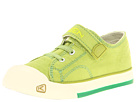
\includegraphics[scale=1]{Fig1/pair3A.jpg}};

	% topconv1 layer
	\node (tconv1) at (5.1cm, 1cm) {};
	\draw [fill=blue!20] (5.4cm,2.9cm) rectangle (9.4cm,-0.1cm);
	\draw [fill=blue!20] (5.2cm,2.7cm) rectangle (9.2cm,-0.3cm);
	\draw [fill=blue!20] (5cm,2.5cm) rectangle (9cm,-0.5cm);

	% arrows from images to conv1s
	\path [draw, ->, line width=3] (im1.east) -- node [above, scale=3] {$I_k$} (tconv1);

	% topconv2 layer
	\node (tconv2) at (12cm, 1cm) {};
	\draw [fill=blue!20] (12.6cm,3.1cm) rectangle (16.6cm,0.1cm);
	\draw [fill=blue!20] (12.4cm,2.9cm) rectangle (16.4cm,-0.1cm);
	\draw [fill=blue!20] (12.2cm,2.7cm) rectangle (16.2cm,-0.3cm);
	\draw [fill=blue!20] (12cm,2.5cm) rectangle (16cm,-0.5cm);

	\path (tconv1.east)+(4.65cm, 0cm) -- node [scale=4]{\dots} (tconv2);

	% toprank
	\node (tconvout) at (16.6cm, 1cm) {};
	
	\node (trank) at (21.5cm, 1cm) [rectangle, draw, fill=red!20, scale=3, align=center] {Ranking \\  Layer};
	\path [draw, line width=3, ->] (tconvout) -- node[above, scale=3] {$\psi_k$} (trank.west);
	
	% posterior
	\node (posterior) at (26.5cm, 1cm){};

	% connect rank layer to posterior
	\path [draw, line width=3, ->] (trank.east) -- node [scale=3, above] {$r_k$} (posterior);

	
\end{tikzpicture}}
\caption{During testing, we only need to evaluate $r_k$ for each test image. Using this value, we can easily infer the relative or absolute ordering of test images, regarding the attribute of interest.} %we have trained our model on.}
\label{fig.4}
\end{figure}
%%%%%%%%%%%%%%%%%%%%%%%% Figure 4 %%%%%%%%%%%%%%%%%%%%%%%%%%%%%%%%%%%%%%%%%%%%%%%%%%%%%

Our proposed model is depicted in figure \ref{fig.3}. The model is trained separately, for each attribute. During training, pairs of images $(I_i, I_j)$ are presented to the network, together with the target probability $t_{ij}$. If for the attribute $I_i \triangleright I_j$ (image $i$ exhibits more of the attribute than image $j$), then $t_{ij}$ is expected to be larger than $0.5$ depending on our confidence on the relative ordering of $I_i$ and $I_j$. Similarly, if $I_i \triangleleft I_j$, then $t_{ij}$ is expected to be smaller than $0.5$, and if it is desired that the two images have the same rank, $t_{ij}$ is expected to be $0.5$. Because of the nature of the datasets, we chose $t_{ij}$ from the set $\{1, 0.5, 0 \}$, according to the available annotations in the dataset.

The pair of images then go though the feature learning and extraction part of the network (ConvNet). This procedure maps the images %into
onto feature vectors $\psi_i$ and $\psi_j$, respectively. Afterwards, these feature vectors go through the ranking layer, as described in section \ref{sec3.1}. We choose the ranking layer to be a fully connected neural network layer with linear activation function, a single output neuron and weights $w$ and $b$. It maps the feature vector $\psi_i$ to the estimated absolute rank of that feature vector $r_i$, where

\begin{equation}
r_i := w^T \psi_i + b
\end{equation}

and $r_i \in \mathbb{R}$.
The two estimated ranks $r_i$ and $r_j$ are then combined to output the estimated posterior probability $ p_{ij} = P(I_i \triangleright I_j)$, %and 
which is used along with the target probability $t_{ij}$ to calculate the loss. This loss is then back-propagated through the network and is used to update the weights of the whole network, including both the weights of the feature learning and extraction sub-network and the ranking layer.

During testing, %test time,
as shown in Figure \ref{fig.4}, we only need to calculate the estimated absolute rank $r_k$ for each test image $I_k$. Using these estimated absolute ranks we can then easily infer the relative or absolute attribute ordering, for all test pairs.

% !TeX root=arXiv.tex
% !TEX TS-program = pdfLatex

%%%%%%%%%%%%%%%%%%%%% EXPERIMENTS %%%%%%%%%%%%%%%%%%%%%%%%%%%%%%%%%%%%%
\section{Experiments}\label{sec.4}

To evaluate our proposed method, we compare it quantitatively with the state-of-the art methods, as well as an informative baseline on all publicly available benchmarks for relative attributes to our knowledge. Furthermore, we perform multiple qualitative experiments to show the ability and superiority of our method.

\subsection{Datasets}\label{sec.4.1}

To assess the performance of the proposed method, we have evaluated it on all publicly available datasets to our knowledge: \textbf{Zappos50K} \cite{Yu2014} (both coarse and fine-grained versions), \textbf{LFW-10} \cite{Sandeep_2014_CVPR} and for the sake of completeness and comparison with previous works, on \textbf{PubFig} and \textbf{OSR} datasets of \cite{parikh2011}.

\textbf{UT-Zap50K} \cite{Yu2014} dataset is a collection of images with annotations for relative comparison of 4 attributes. This dataset contains two collections: Zappos50K-1 where relative attributes are annotated for coarse pairs where the comparison is relatively easy to make, and Zappos50K-2 where relative attributes are annotated for fine-grained pairs for which making the distinction between them is hard according to human annotators.
Training set for Zappos50K-1 contains approximately 1500 to 1800 annotated pairs of images for each attribute. These are divided into 10 train/test splits which are provided alongside the dataset and used in this work. Meanwhile, Zappos50K-2 only contains a test set of approximately 4300 pairs, and for training the set of images in Zappos50K-1 are used.
% This dataset consists of two collections, namely UT-Zap50K-1, in which \textit{coarse} relative attributes are compared for image pairs, and UT-Zap50K-2, in which \textit{fine-grained} relative attributes are compared for image pairs.

We have also conducted experiments on the \textbf{LFW-10} \cite{Sandeep_2014_CVPR} dataset. This dataset has 2000 images of faces of people and annotations for 10 attributes. For each attribute, a random subset of 500 pairs of images have been annotated for each train and test set.
% These two latter datasets have large number of categories, as well as large inter-sample varieties in terms of poses, lighting condition. This makes them quite challenging compared to PubFig and OSR.

\textbf{PubFig} \cite{parikh2011} dataset (a set of public figure faces), consists of 800 facial images of 8 random subjects, with 11 attributes.
\textbf{OSR} \cite{parikh2011} dataset contains 2688 images of outdoor scenes in 8 categories, for which 6 relative attributes are defined.
The ordering of samples in both PubFig and OSR datasets are annotated in a category level, \ie, all images in a specific category may be ranked higher, equal, or lower than all images in another category, with respect to an attribute. This sometimes causes annotation inconsistencies \cite{Sandeep_2014_CVPR}.
In our experiments, we have used the provided train/test split of PubFig and OSR datasets.


\subsection{Experimental setup}
We train our proposed model (described in Section \ref{sec.3}) for each attribute, separately. While it is possible  to train multiple attributes at the same time, however, this is not done due to the structure of datasets, where for each training pair of images only a certain attribute is annotated.

We have used the Lasagne \cite{lasagne} deep learning framework to to implement our model.
In all our experiments, for the feature learning and extraction part of the network,
%we use layer fc7 of VGG-16 model of \cite{verydeep} (the last layer before the probability layer).
we use the VGG-16 model of \cite{verydeep} and trim out the probability layer (all layers up to fc7 are used but the probability layer is not included).
We initialize the weights of the model using a pretrained model on ILSVRC 2014 dataset \cite{ilsvrc2014} for the task of image classification. These weights get fine-tuned as the network learns to predict the relative attributes (see section \ref{sec.qres}). The weights $w$ of the ranking layer are initialized using the Xavier method \cite{glorot}, and the bias is initialized to 0.

For training, we use stochastic gradient descent with RMSProp \cite{Tieleman2012} updates and minibatches of size 32 (16 pair of images).
We set the learning rate for all experiments to $10^{-4}$ (for all weights and biases both the feature learning and extraction layers and the ranking layer), initially, then RMSProp changes the learning rates according to its algorithm. We have also used weight decay ($\ell_2$ norm regularization), with a fixed $0.005$ multiplier. Furthermore when calculating the binary cross entropy loss we clip the estimated posterior $p_{ij}$ to be in the range $[10^{-7}, 1 - 10^{-7}]$. This is used to prevent the loss from diverging.

In each epoch, we randomly shuffle the training pairs. The number of epochs of training were chosen to reflect the training size. For Zappos50K and LFW-10 datasets, we train for 5 and 50 epochs, respectively. For PubFig and OSR datasets, we train for 120 epochs due to the small number of training samples. Also we have added random horizontal flipping of the training images as a way to augment the training set for the PubFig and OSR datasets.

\subsection{Baseline}

As a baseline, we have also included results for the RankSVM method (as in \cite{parikh2011}), when the features given to the method were computed from the output of the VGG-16 pretrained network on ILSVRC 2014. 

Using this baseline we can evaluate the extent of effectiveness of off-the-shelf ConvNet features \cite{offtheshelf}  for the task of ranking. In a sense, comparing this baseline with our proposed method reveals the effect of features fine-tuning, for the task. 

\subsection{Quantitative Results}

Following \cite{parikh2011, Yu2014, Sandeep_2014_CVPR}, we report the accuracy in terms of the percentage of correctly ordered pairs. For our proposed method, we report the mean accuracy and standard deviation over 3 separate runs. 
%For a complete report on the results including the standard deviation of the results see supplementary materials.

Table \ref{tab:osr} shows our results on the OSR dataset. Our method outperforms the baseline and the state-of-the-art on this dataset, on all attributes except for `Natural' attribute, where the baseline outperforms our method with a small margin. One possible cause of this could be that the pretrained network of the baseline is still appropriate for this dataset, since the dataset contains natural images. This is a relatively easy dataset, and we would assume that it cannot show the ability of our method to learn better features.

%%%%%%%%%%%%%%%%%%%%%% OSR RESULTS %%%%%%%%%%%%%%%%%%%%%
\begin{table*}[t!]
\caption{Results for the OSR dataset}
\centering
\resizebox{2\columnwidth}{!}{
\begin{tabular}{l| c | c | c | c | c | c | c }
\textbf{Method} & \textbf{Natural} & \textbf{Open} &  \textbf{Perspective} & \textbf{Large Size} & \textbf{Diag} & \textbf{ClsDepth} & \textbf{Mean}\\ \hline
 Relative Attributes~\cite{parikh2011} &  95.03 & 90.77 & 86.73 & 86.23 & 86.50 & 87.53 & 88.80 \\
 Relative Forest~\cite{Li2013} & 95.24 & 92.39 & 87.58 & 88.34 & 89.34 & 89.54 & 90.41 \\
 Fine-grained Comparison~\cite{Yu2014} & 95.70 & 94.10 & 90.43 & 91.10 & 92.43 & 90.47 & 92.37 \\
 VGG16-fc7 (baseline) & 97.98 & 87.82 & 89.01 & 88.25 & 89.91 & 90.70 & 90.61 \\
 %RankNet (ours) & 97.76 ($\pm$ 0.25) & 94.48 ($\pm$ 0.90) & 92.37 ($\pm$ 0.34) & 92.70 ($\pm$ 1.01) & 95.14 ($\pm$ 0.26) & 91.44 ($\pm$ 2.69) & \textbf{93.98} ($\pm$ 0.35) \\
 \hline
 \multirow{2}{*}{RankNet (ours)} & 97.76  & 94.48  & 92.37  & 92.70  & 95.14  & 91.44  & \textbf{93.98}  \\
        & \scriptsize{($\pm$ 0.25)} & \scriptsize{($\pm$ 0.90)} & \scriptsize{($\pm$ 0.34)} & \scriptsize{($\pm$ 1.01)} & \scriptsize{($\pm$ 0.26)} & \scriptsize{($\pm$ 2.69)} & \scriptsize{($\pm$ 0.35)} \\
 \hline
\end{tabular}}
\label{tab:osr}
\end{table*}
%%%%%%%%%%%%%%%%%%%%%%%%%%%%%%%%%%%%%%%%%%%%%%%%%%%%%%%%%

Table \ref{tab:pubfig} shows our results on the PubFig dataset. On this dataset, our results are very competitive with the state-of-the-art. We think this is due to label inconsistency in this dataset, low number of training samples, and the fact that the images in the dataset are very tightly cropped to the face. This makes the decision about the attributes very local, while our method performs the ranking and feature extraction in a global manner.

%%%%%%%%%%%%%%%%%%%%%% PUBFIG RESULTS %%%%%%%%%%%%%%%%%%%
\begin{table*}[t!]
\caption{Results for the PubFig dataset}
\centering
\resizebox{2\columnwidth}{!}{
\begin{tabular}{l|c|c|c|c|c|c|c|c|c|c|c|c}
 \textbf{Method} & \textbf{Male} & \textbf{White} & \textbf{Young} & \textbf{Smiling} & \textbf{Chubby} & \textbf{Forehead} & \textbf{Eyebrow} & \textbf{Eye} & \textbf{Nose} & \textbf{Lip} & \textbf{Face} & \textbf{Mean}  \\ \hline
 Relative Attributes~\cite{parikh2011} & 81.80 & 76.97 & 83.20 & 79.90 & 76.27 & 87.60 & 79.87 & 81.67 & 77.40 & 79.17 & 82.33 & 80.53 \\ 
 Relative Forest~\cite{Li2013} & 85.33 & 82.59 & 84.41 & 83.36 & 78.97 & 88.83 & 81.84 & 83.15 & 80.43 & 81.87 & 86.31 & 83.37 \\
 Fine-grained Comparison~\cite{Yu2014} & 91.77 & 87.43 & 91.87 & 87.00 & 87.37 & 94.00 & 89.83 & 91.40 & 89.07 & 90.43 & 86.70 & \textbf{89.72} \\
 VGG16-fc7 (baseline) & 80.84 & 73.39 & 79.41 & 76.23 & 74.69 & 80.52 & 75.38 & 77.78 & 76.15 & 78.14 & 80.01 & 77.50 \\
 %RankNet (ours) & \pbox{20cm}{\centering 90.10\\($\pm$ 1.05)} & 89.49 ($\pm$ 0.59) & 89.83 ($\pm$ 0.37) & 88.62 ($\pm$ 1.59) & 88.72 ($\pm$ 0.75) & 9.33 ($\pm$ 0.80) & 88.13 ($\pm$ 1.83) & 86.94 ($\pm$ 3.36) & 86.30 ($\pm$ 1.60) & 89.79 ($\pm$ 0.45) & 92.71 ($\pm$ 1.87) & \textbf{89.36 ($\pm$ 0.57)} \\
 \hline
 \multirow{2}{*}{RankNet (ours)} & 90.10 & 89.49 & 89.83 & 88.62 & 88.72 & 92.33 & 88.13 & 86.94 & 86.30 & 89.79 & 92.71 & \textbf{89.36} \\
                                 & \scriptsize{($\pm$ 1.05)} & \scriptsize{($\pm$ 0.59)} & \scriptsize{($\pm$ 0.37)} & \scriptsize{($\pm$ 1.59)} & \scriptsize{($\pm$ 0.75)} & \scriptsize{($\pm$ 0.80)} &  \scriptsize{($\pm$ 1.83)} & \scriptsize{($\pm$ 3.36)} & \scriptsize{($\pm$ 1.60)} & \scriptsize{($\pm$ 0.45)} & \scriptsize{($\pm$ 1.87)} & \scriptsize{($\pm$ 0.57)} \\
 \hline
\end{tabular}}
\label{tab:pubfig}
\end{table*}
%%%%%%%%%%%%%%%%%%%%%%%%%%%%%%%%%%%%%%%%%%%%%%%%%%%%%%%%

Table \ref{tab:lfw} shows our results on the LFW-10 dataset. On this dataset, our method outperforms the state-of-the-art by a large margin. Meanwhile, the baseline cannot achieve a comparative result. This shows that for achieving good results, the feature learning part have had a large impact.

%%%%%%%%%%%%%%%%%%%%%%% LFW-10 RESULTS %%%%%%%%%%%%%%%%%%
\begin{table*}[t!]
\caption{Results for the LFW-10 dataset}
\centering
\resizebox{2\columnwidth}{!}{
\begin{tabular}{l|c|c|c|c|c|c|c|c|c|c|c}
 \textbf{Method} & \textbf{Bald} & \textbf{DkHair} & \textbf{Eyes} & \textbf{GdLook} & \textbf{Mascu.} & \textbf{Mouth} & \textbf{Smile} & \textbf{Teeth} & \textbf{FrHead} & \textbf{Young} & \textbf{Mean} \\ \hline
 Fine-grained Comparison~\cite{Li2013} & 67.9 & 73.6 & 49.6 & 64.7 & 70.1 & 53.4 & 59.7 & 53.5 & 65.6 & 66.2 & 62.4  \\
 Relative Attributes~\cite{parikh2011} & 70.4 & 75.7 & 52.6 & 68.4 & 71.3 & 55.0 & 54.6 & 56.0 & 64.5 & 65.8 & 63.4 \\
 Relative Parts~\cite{Sandeep_2014_CVPR} & 71.8 & 80.5 & 90.5 & 77.6 & 67.0 & 77.6 & 81.3 & 76.2 & 80.2 & 82.4 & 78.5 \\
 Global + HOG~\cite{vermaexploring} & 78.8 & 72.4 & 70.7 & 67.6 & 84.5 & 67.8 & 67.4 & 71.7 & 79.3 & 68.4 & 72.9 \\
 VGG16-fc7 (baseline) & 70.44 & 69.14 & 59.40 & 59.75 & 84.48 & 56.04 & 57.63 & 57.85 & 59.38 & 70.36 & 64.45 \\
 \hline
 \multirow{2}{*}{RankNet (ours)} & 81.27 & 88.92 & 91.98 & 72.03 & 95.40 & 89.04 & 84.75 & 89.33 & 84.11 & 73.35 & \textbf{85.02} \\ 
                                 & \scriptsize{($\pm$ 1.47)} & \scriptsize{($\pm$ 1.63)} & \scriptsize{($\pm$ 2.42)} & \scriptsize{($\pm$ 1.25)} & \scriptsize{($\pm$ 1.52)} & \scriptsize{($\pm$ 2.18)} & \scriptsize{($\pm$ 0.28)} & \scriptsize{($\pm$ 0.47)} & \scriptsize{($\pm$ 2.77)} & \scriptsize{($\pm$ 1.13)} & \scriptsize{($\pm$ 0.59)} \\
 \hline
\end{tabular}}
\label{tab:lfw}
\end{table*}
%%%%%%%%%%%%%%%%%%%%%%%%%%%%%%%%%%%%%%%%%%%%%%%%%%%%%%%%

Tables \ref{tab:zap1} and \ref{tab:zap2} show the results on Zappos50K-1 and Zappos50K-2 datasets, respectively. Our method, again, achieves the state-of-the-art accuracy on both fine-grained and coarse datasets. However, our baseline method does not achieve a good result on this dataset. We think this is due to the fact that the images in the Zappos50K dataset are not natural images. So the extracted features in the baseline method are not appropriate for ranking. But our proposed method learns appropriate features for the task, given the large amount of training data available in this dataset.

%%%%%%%%%%%%%%%%%%%%%% Zap50K-1 RESULTS %%%%%%%%%%%%%%%%
\begin{table}[h]
\caption{Results for the UT-Zap50K-1 (coarse) dataset}
%\centering
\resizebox{1\columnwidth}{!}{
\begin{tabular}{l|c|c|c|c|c}
 \textbf{Method} & \textbf{Open} & \textbf{Pointy} & \textbf{Sporty} & \textbf{Comfort} & \textbf{Mean} \\ \hline
 Relative Attributes~\cite{parikh2011} & 87.77 & 89.37 & 91.20 & 89.93 & 89.57 \\
 Fine-grained Comparison~\cite{Yu2014} & 90.67 & 90.83 & 92.67 & 92.37 & 91.64 \\
 VGG16-fc7 (baseline) & 62.33 & 59.57 & 61.33 & 61.00 & 61.08 \\
 \hline
 \multirow{2}{*}{RankNet (ours)} & 93.00 & 92.11 & 95.56 & 93.22 & \textbf{93.47}\\
                                 & \scriptsize{($\pm$ 1.15)} & \scriptsize{($\pm$ 1.58)} & \scriptsize{($\pm$ 1.26)} & \scriptsize{($\pm$ 2.41)} & \scriptsize{($\pm$ 0.59)}\\
 \hline
\end{tabular}}
\label{tab:zap1}
\end{table}
%%%%%%%%%%%%%%%%%%%%%%%%%%%%%%%%%%%%%%%%%%%%%%%%%%%%%%%%


%%%%%%%%%%%%%%%%%%%%%% Zap50K-2 RESULTS %%%%%%%%%%%%%%%%
\begin{table}[h]
\caption{Results for the UT-Zap50K-2 (fine-grained) dataset}
%\centering
\resizebox{\columnwidth}{!}{
\begin{tabular}{l|c|c|c|c|c}
 \textbf{Method} & \textbf{Open} & \textbf{Pointy} & \textbf{Sporty} & \textbf{Comfort} & \textbf{Mean} \\ \hline
 Relative Attributes~\cite{parikh2011} & 60.18 & 59.56 & 62.70 & 64.04 & 61.62  \\
 Fine-grained Comparison~\cite{Yu2014} & 74.91 & 63.74 & 64.54 & 62.51 & 66.43  \\
 LocalPair + ML + HOG~\cite{vermaexploring} & 76.2 & 65.3 & 64.8 & 63.6 & 67.5 \\
 VGG16-fc7 (baseline) & 52.55 & 52.65 & 51.52 & 53.01 & 52.43 \\
 \hline
 \multirow{2}{*}{RankNet (ours)} & 71.21 & 66.64 & 67.81 & 65.88 & \textbf{67.88} \\
                                 & \scriptsize{($\pm$ 1.50)} & \scriptsize{($\pm$ 1.81)} & \scriptsize{($\pm$ 0.84)} & \scriptsize{($\pm$ 1.92)} & \scriptsize{($\pm$ 0.83)}\\
 \hline
\end{tabular}}
\label{tab:zap2}
\end{table}
%%%%%%%%%%%%%%%%%%%%%%%%%%%%%%%%%%%%%%%%%%%%%%%%%%%%%%%%

\subsection{Qualitative Results} \label{sec.qres}


%%%%%%%%%%%%%%%%%%%%% Figure featspace %%%%%%%%%%%%%%%%%%%%%%%%%%%%%%%%
\begin{figure*}
\resizebox{2\columnwidth}{!}{
\centering
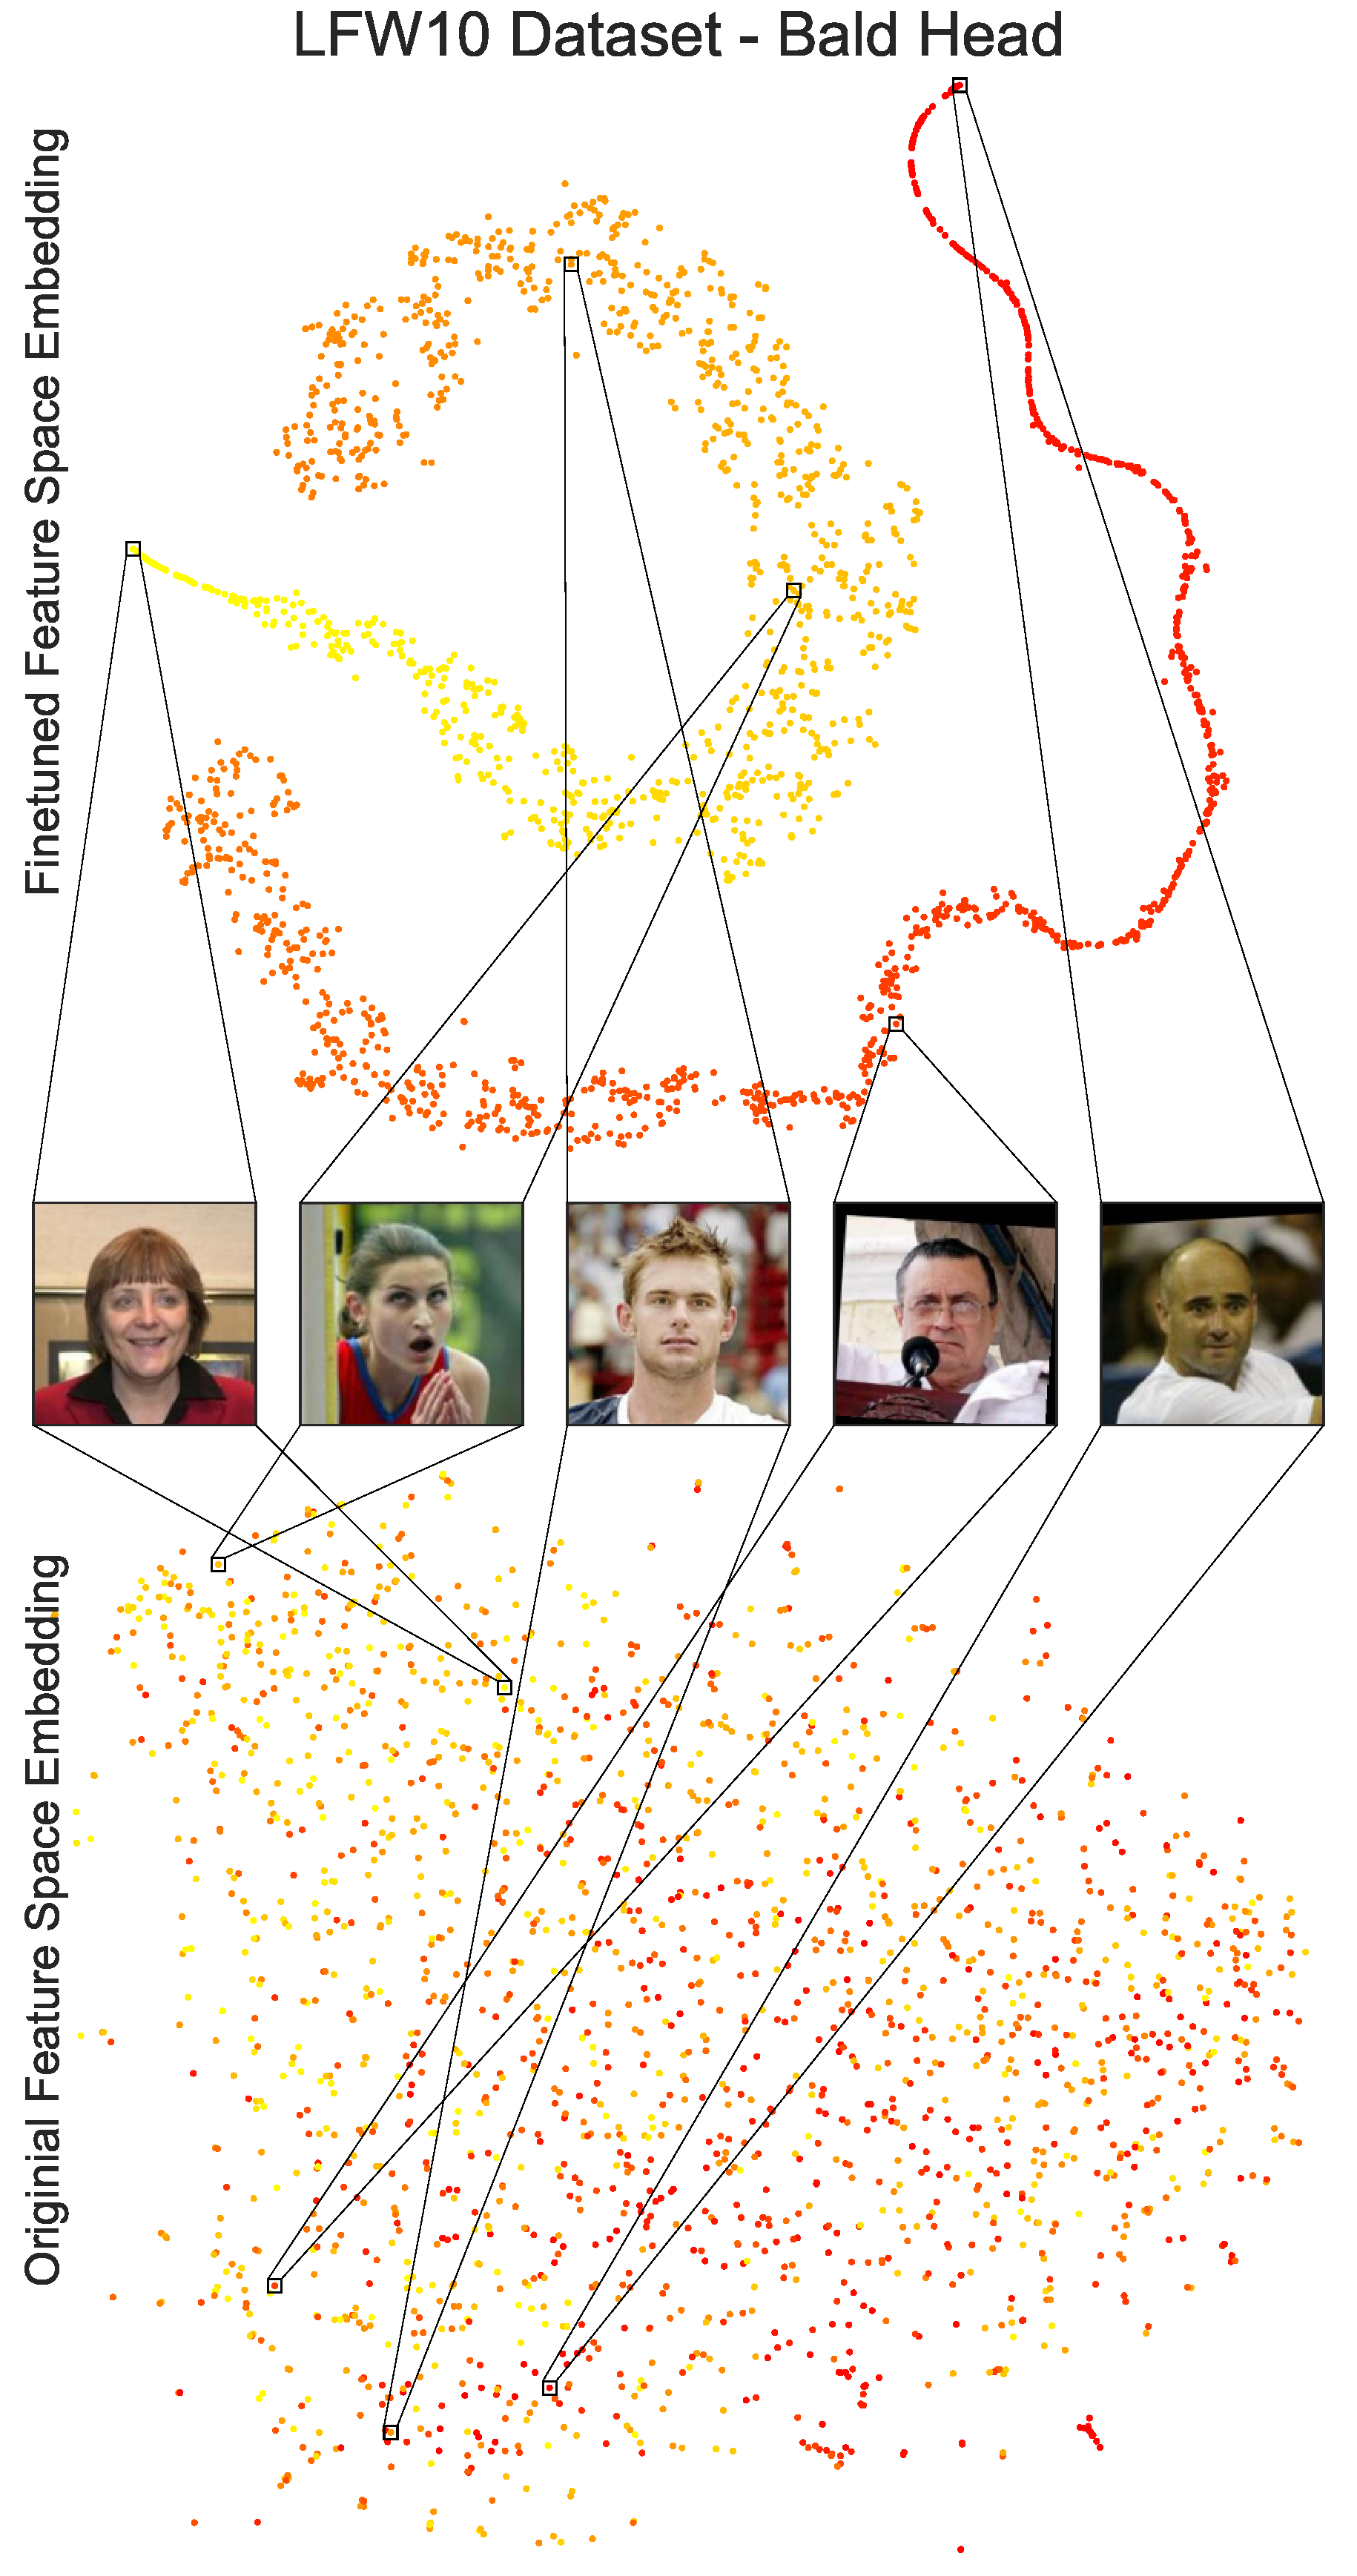
\includegraphics{lfw10-baldhead-featspace.pdf}
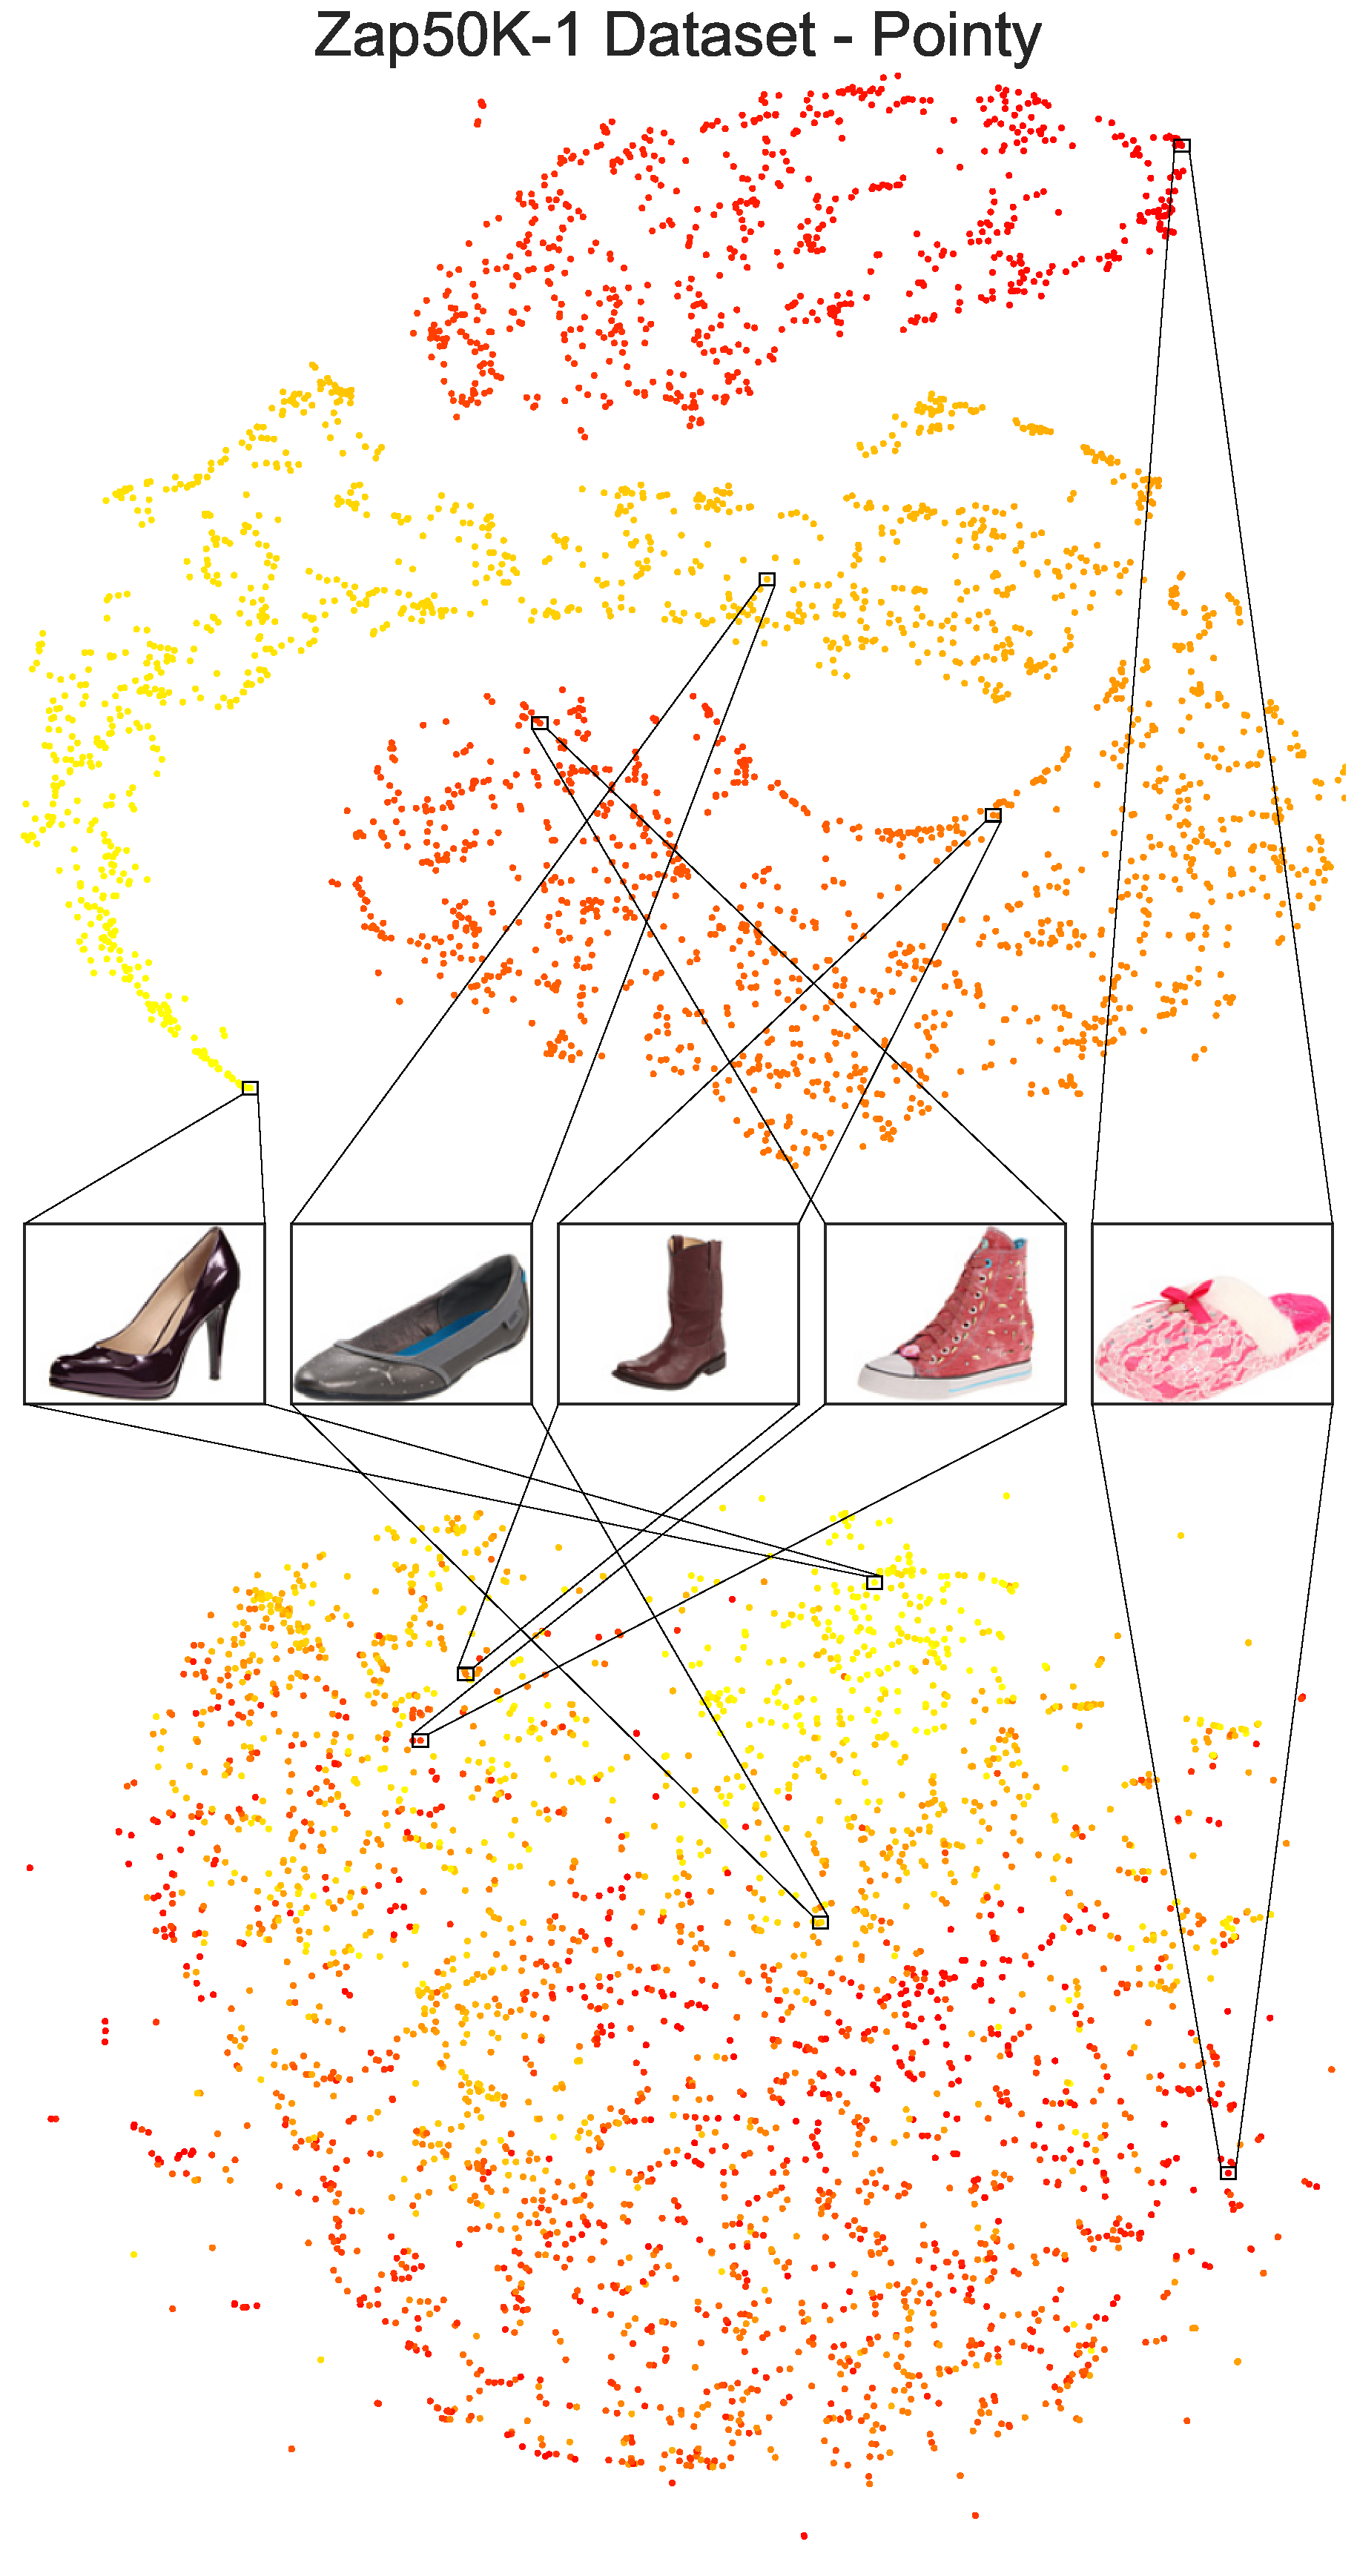
\includegraphics{zappos-pointy-featspace.pdf}
}
\caption{t-SNE embedding of images in fine-tuned feature space (top) and original feature space (bottom). The set of visualizations on the left are for the \textit{Bald Head} attribute of the LFW-10 dataset. The set of visualizations on the right are for the \textit{Pointy} attribute of the Zappos50K-1 dataset. Images in the middle row show a number of samples from the feature space. It is clear that images are ordered according to their value of the attribute. Each point is colored according to its value of the respective attribute, to discriminate images according to their value of the attribute.}
\label{featspace}
\end{figure*}
%%%%%%%%%%%%%%%%%%%%% Figure featspace %%%%%%%%%%%%%%%%%%%%%%%%%%%%%%%%


%%%%%%%%%%%%%%%%%%%%% Figure 5 %%%%%%%%%%%%%%%%%%%%%%%%%%%%%%%%%%%%%%%%
\begin{figure*}
\scalebox{.38}
{
\begin{tikzpicture}

		\node [scale=2] (strong) {\textit{strong}}; 
	\node [scale=2, right=31cm of strong] (weak) {\textit{weak}};
	\path [draw, line width=3, <->, blue] (strong.south west) -- (weak.south east);

	% attr1
	\node [below=0.5cm of strong] (attr1im1) {
\includegraphics[width=4cm, height=4cm]{spectrum/attr1/im1.jpg}};
	\node (attr1name) [scale=2, left=0.5cm of attr1im1] {Smile (LFW-10)};
	\node [right=0.5cm of attr1im1] (attr1im2) {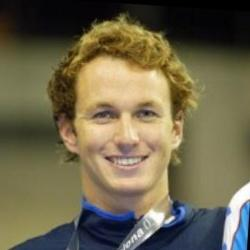
\includegraphics[width=4cm, height=4cm]{spectrum/attr1/im2.jpg}};
	\node [right=0.5cm of attr1im2] (attr1im3) {
\includegraphics[width=4cm, height=4cm]{spectrum/attr1/im3.jpg}};
	\node [right=0.5cm of attr1im3] (attr1im4) {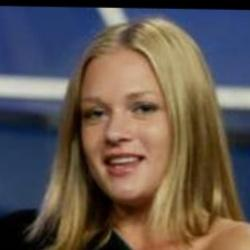
\includegraphics[width=4cm, height=4cm]{spectrum/attr1/im4.jpg}};
	\node [right=0.5cm of attr1im4] (attr1im5) {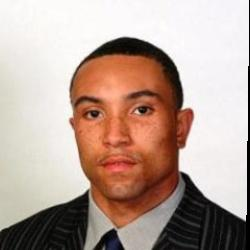
\includegraphics[width=4cm, height=4cm]{spectrum/attr1/im5.jpg}};
	\node [right=0.5cm of attr1im5] (attr1im6) {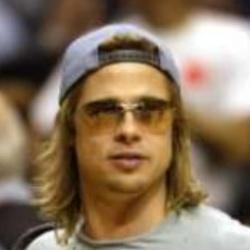
\includegraphics[width=4cm, height=4cm]{spectrum/attr1/im6.jpg}};
	\node [right=0.5cm of attr1im6] (attr1im7) {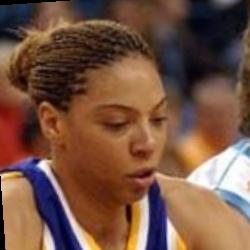
\includegraphics[width=4cm, height=4cm]{spectrum/attr1/im7.jpg}};
	\node [right=0.5cm of attr1im7] (attr1im8) {
\includegraphics[width=4cm, height=4cm]{spectrum/attr1/im8.jpg}};

% 	% attr2
% 	\node [below=0.5cm of attr1im1] (attr2im1) {
\includegraphics[width=4cm, height=4cm]{spectrum/attr2/im1.jpg}};
% 	\node (attr2name) [scale=2, left=0.5cm of attr2im1] {Young};
% 	\node [right=0.5cm of attr2im1] (attr2im2) {
\includegraphics[width=4cm, height=4cm]{spectrum/attr2/im2.jpg}};
% 	\node [right=0.5cm of attr2im2] (attr2im3) {
\includegraphics[width=4cm, height=4cm]{spectrum/attr2/im3.jpg}};
% 	\node [right=0.5cm of attr2im3] (attr2im4) {
\includegraphics[width=4cm, height=4cm]{spectrum/attr2/im4.jpg}};
% 	\node [right=0.5cm of attr2im4] (attr2im5) {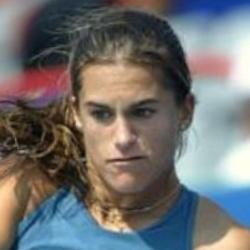
\includegraphics[width=4cm, height=4cm]{spectrum/attr2/im5.jpg}};
% 	\node [right=0.5cm of attr2im5] (attr2im6) {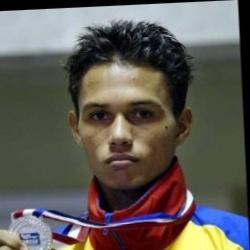
\includegraphics[width=4cm, height=4cm]{spectrum/attr2/im6.jpg}};
% 	\node [right=0.5cm of attr2im6] (attr2im7) {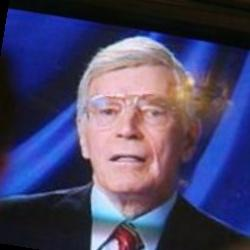
\includegraphics[width=4cm, height=4cm]{spectrum/attr2/im7.jpg}};
% 	\node [right=0.5cm of attr2im7] (attr2im8) {
\includegraphics[width=4cm, height=4cm]{spectrum/attr2/im8.jpg}};

% 	% attr3
% 	\node [below=0.5cm of attr2im1] (attr3im1) {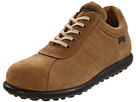
\includegraphics[width=4cm, height=3cm]{spectrum/attr3/im1.jpg}};
% 	\node (attr3name) [scale=2, left=0.5cm of attr3im1] {Comfort};
% 	\node [right=0.5cm of attr3im1] (attr3im2) {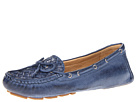
\includegraphics[width=4cm, height=3cm]{spectrum/attr3/im2.jpg}};
% 	\node [right=0.5cm of attr3im2] (attr3im3) {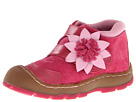
\includegraphics[width=4cm, height=3cm]{spectrum/attr3/im3.jpg}};
% 	\node [right=0.5cm of attr3im3] (attr3im4) {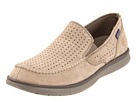
\includegraphics[width=4cm, height=3cm]{spectrum/attr3/im4.jpg}};
% 	\node [right=0.5cm of attr3im4] (attr3im5) {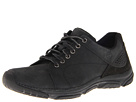
\includegraphics[width=4cm, height=3cm]{spectrum/attr3/im5.jpg}};
% 	\node [right=0.5cm of attr3im5] (attr3im6) {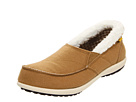
\includegraphics[width=4cm, height=3cm]{spectrum/attr3/im6.jpg}};
% 	\node [right=0.5cm of attr3im6] (attr3im7) {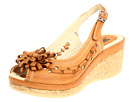
\includegraphics[width=4cm, height=3cm]{spectrum/attr3/im7.jpg}};
% 	\node [right=0.5cm of attr3im7] (attr3im8) {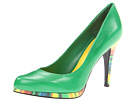
\includegraphics[width=4cm, height=3cm]{spectrum/attr3/im8.jpg}};

	% attr4
	\node [below=0.5cm of attr1im1] (attr4im1) {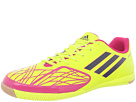
\includegraphics[width=4cm, height=3cm]{spectrum/attr4/im1.jpg}};
	\node (attr4name) [scale=2, left=0.5cm of attr4im1] {Sporty (Zappos50K-1)};
	\node [right=0.5cm of attr4im1] (attr4im2) {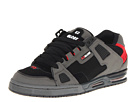
\includegraphics[width=4cm, height=3cm]{spectrum/attr4/im2.jpg}};
	\node [right=0.5cm of attr4im2] (attr4im3) {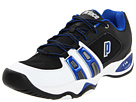
\includegraphics[width=4cm, height=3cm]{spectrum/attr4/im3.jpg}};
	\node [right=0.5cm of attr4im3] (attr4im4) {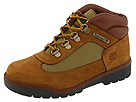
\includegraphics[width=4cm, height=3cm]{spectrum/attr4/im4.jpg}};
	\node [right=0.5cm of attr4im4] (attr4im5) {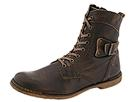
\includegraphics[width=4cm, height=3cm]{spectrum/attr4/im5.jpg}};
	\node [right=0.5cm of attr4im5] (attr4im6) {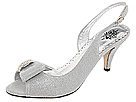
\includegraphics[width=4cm, height=3cm]{spectrum/attr4/im6.jpg}};
	\node [right=0.5cm of attr4im6] (attr4im7) {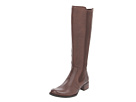
\includegraphics[width=4cm, height=3cm]{spectrum/attr4/im7.jpg}};
	\node [right=0.5cm of attr4im7] (attr4im8) {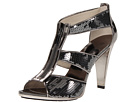
\includegraphics[width=4cm, height=3cm]{spectrum/attr4/im8.jpg}};

	% attr5
	\node [below=0.5cm of attr4im1] (attr5im1) {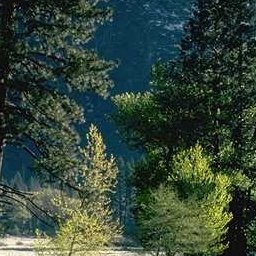
\includegraphics[width=4cm, height=4cm]{spectrum/attr5/im1.jpg}};
	\node (attr5name) [scale=2, left=0.5cm of attr5im1] {Natural (OSR)};
	\node [right=0.5cm of attr5im1] (attr5im2) {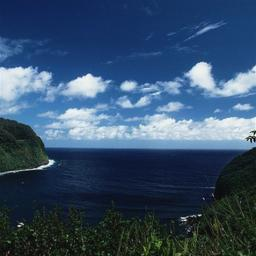
\includegraphics[width=4cm, height=4cm]{spectrum/attr5/im2.jpg}};
	\node [right=0.5cm of attr5im2] (attr5im3) {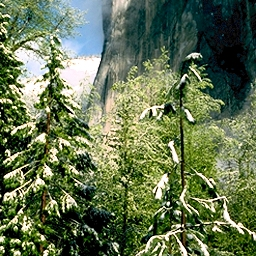
\includegraphics[width=4cm, height=4cm]{spectrum/attr5/im3.jpg}};
	\node [right=0.5cm of attr5im3] (attr5im4) {\includegraphics[width=4cm, height=4cm]{spectrum/attr5/im4.jpg}};
	\node [right=0.5cm of attr5im4] (attr5im5) {\includegraphics[width=4cm, height=4cm]{spectrum/attr5/im5.jpg}};
	\node [right=0.5cm of attr5im5] (attr5im6) {\includegraphics[width=4cm, height=4cm]{spectrum/attr5/im6.jpg}};
	\node [right=0.5cm of attr5im6] (attr5im7) {\includegraphics[width=4cm, height=4cm]{spectrum/attr5/im7.jpg}};
	\node [right=0.5cm of attr5im7] (attr5im8) {\includegraphics[width=4cm, height=4cm]{spectrum/attr5/im8.jpg}};

% 	% attr6
% 	\node [below=0.5cm of attr5im1] (attr6im1) {\includegraphics[width=4cm, height=4cm]{spectrum/attr6/im1.jpg}};
% 	\node (attr6name) [scale=2, left=0.5cm of attr6im1] {Open};
% 	\node [right=0.5cm of attr6im1] (attr6im2) {\includegraphics[width=4cm, height=4cm]{spectrum/attr6/im2.jpg}};
% 	\node [right=0.5cm of attr6im2] (attr6im3) {\includegraphics[width=4cm, height=4cm]{spectrum/attr6/im3.jpg}};
% 	\node [right=0.5cm of attr6im3] (attr6im4) {\includegraphics[width=4cm, height=4cm]{spectrum/attr6/im4.jpg}};
% 	\node [right=0.5cm of attr6im4] (attr6im5) {\includegraphics[width=4cm, height=4cm]{spectrum/attr6/im5.jpg}};
% 	\node [right=0.5cm of attr6im5] (attr6im6) {\includegraphics[width=4cm, height=4cm]{spectrum/attr6/im6.jpg}};
% 	\node [right=0.5cm of attr6im6] (attr6im7) {\includegraphics[width=4cm, height=4cm]{spectrum/attr6/im7.jpg}};
% 	\node [right=0.5cm of attr6im7] (attr6im8) {\includegraphics[width=4cm, height=4cm]{spectrum/attr6/im8.jpg}};

	% attr7
	\node [below=0.5cm of attr5im1] (attr7im1) {\includegraphics[width=4cm, height=4cm]{spectrum/attr7/im1.jpg}};
	\node (attr7name) [scale=2, left=0.5cm of attr7im1] {Forehead (PubFig)};
	\node [right=0.5cm of attr7im1] (attr7im2) {\includegraphics[width=4cm, height=4cm]{spectrum/attr7/im2.jpg}};
	\node [right=0.5cm of attr7im2] (attr7im3) {\includegraphics[width=4cm, height=4cm]{spectrum/attr7/im3.jpg}};
	\node [right=0.5cm of attr7im3] (attr7im4) {\includegraphics[width=4cm, height=4cm]{spectrum/attr7/im4.jpg}};
	\node [right=0.5cm of attr7im4] (attr7im5) {\includegraphics[width=4cm, height=4cm]{spectrum/attr7/im5.jpg}};
	\node [right=0.5cm of attr7im5] (attr7im6) {\includegraphics[width=4cm, height=4cm]{spectrum/attr8/im2.jpg}};
	\node [right=0.5cm of attr7im6] (attr7im7) {\includegraphics[width=4cm, height=4cm]{spectrum/attr7/im7.jpg}};
	\node [right=0.5cm of attr7im7] (attr7im8) {\includegraphics[width=4cm, height=4cm]{spectrum/attr7/im8.jpg}};

% 	% attr8
% 	\node [below=0.5cm of attr7im1] (attr8im1) {\includegraphics[width=4cm, height=4cm]{spectrum/attr8/im1.jpg}};
% 	\node (attr8name) [scale=2, left=0.5cm of attr8im1] {Open Eyes};
% 	\node [right=0.5cm of attr8im1] (attr8im2) {\includegraphics[width=4cm, height=4cm]{spectrum/attr8/im2.jpg}};
% 	\node [right=0.5cm of attr8im2] (attr8im3) {\includegraphics[width=4cm, height=4cm]{spectrum/attr8/im3.jpg}};
% 	\node [right=0.5cm of attr8im3] (attr8im4) {\includegraphics[width=4cm, height=4cm]{spectrum/attr8/im4.jpg}};
% 	\node [right=0.5cm of attr8im4] (attr8im5) {\includegraphics[width=4cm, height=4cm]{spectrum/attr8/im5.jpg}};
% 	\node [right=0.5cm of attr8im5] (attr8im6) {\includegraphics[width=4cm, height=4cm]{spectrum/attr8/im6.jpg}};
% 	\node [right=0.5cm of attr8im6] (attr8im7) {\includegraphics[width=4cm, height=4cm]{spectrum/attr8/im7.jpg}};
% 	\node [right=0.5cm of attr8im7] (attr8im8) {\includegraphics[width=4cm, height=4cm]{spectrum/attr8/im8.jpg}};
\end{tikzpicture}}
\caption{Images are ordered according to the value of their respective attributes.}
\label{figspectrum}
\end{figure*}
%%%%%%%%%%%%%%%%%%%%% Figure 5 %%%%%%%%%%%%%%%%%%%%%%%%%%%%%%%%%%%%%%%%

Our proposed method uses a deep network with two parts, the feature learning and extraction part and the ranking part. During training, not only the weights for the ranking part are learned, but also the weights for the feature learning and extraction part of the network, which were initialized using a pretrained network, are fine-tuned. By fine-tuning the features, our network learns a set of features that are more appropriate for the images of that particular dataset and attribute. To show the effectiveness of fine-tuning the features of the feature learning and extraction part of the network, we have projected them into 2-D space using the t-SNE \cite{van2008visualizing} method, as can be seen in Figure \ref{featspace}. The visualizations on the top of each figure show the images projected into 2-D space from the fine-tuned feature space. Each image is displayed as a point. It is clear from these visualizations that fine-tuned feature space is better in capturing the ordering of images with respect to the respective attribute. Since t-SNE embedding is a non-linear embedding, relative distances between points in the high-dimensional space and the low-dimensional embedding space are preserved, thus close points in the low-dimensional embedding space are also close to each other in the high-dimensional space. It can therefore be seen that fine-tuning indeed changes the feature space such that images with similar values of the respective attribute get projected into a close vicinity of the feature space. However, in the original feature space, images are projected according to their visual content, regardless of their value of the attribute.

Another property of our network is that it can achieve a total ordering of images, given a set of pairwise orderings. In spite of the fact that training samples are pairs of images annotated according to their relative value of the attribute, the network can generalize the relativity of attribute values to other pairs of images. Figure \ref{figspectrum} shows that images can be ordered according to their value of the respective attribute. 

\subsection{Saliency Maps and Localizing the Attributes} \label{sec.4.5}

We have also used the method of \cite{saliency} to visualize the saliency of each attribute. Giving two image as inputs to the network we take the derivative of the estimated posterior with respect to the input images and visualize them. Figure \ref{fig.5} shows some sample visualization for the LFW-10 dataset's test pairs. To generate this figure we have have applied Gaussian smoothing to the saliency map.
Using this visualization we can localize the attribute using the same network that was trained to rank the attributes in an unsupervised manner, \ie, although we haven't explicitly trained our network to localize the salient and informative regions of the image, however, it has implicitly learned to find these regions. We see that this technique is able to localize both easy attributes such as "Open Eyes" and abstract attributes such as "Good Looking". Our approach reveals some interesting properties about salient pixels for each attribute. For example, for the attribute "Open Eyes", not only pixels belonging to the eye are salient, but also the pixels which belong to the mouth are salient, because the person with open mouth usually has open eyes.

\begin{figure}
\captionsetup[subfigure]{labelformat=empty}
    \centering
    \begin{subfigure}
        \centering
        \includegraphics[width=8cm, trim={0 1cm 0 0},clip]{saliency-new/saliency-smooth/bald-1.jpeg}
        \footnotesize
        \stackunder[3pt]{
            \includegraphics[width=8cm, trim={0 0 0 1cm},clip]{saliency-new/saliency-smooth/bald-6.jpeg}
        }{Bald Head}
        \vspace{0.4cm}
    \end{subfigure}
    
    \begin{subfigure}
        \centering
        \includegraphics[width=8cm, trim={0 1cm 0 0},clip]{saliency-new/saliency-smooth/smile-1.jpeg}
        \footnotesize
        \stackunder[3pt]{
            \includegraphics[width=8cm, trim={0 0 0 1cm},clip]{saliency-new/saliency-smooth/smile-4.jpeg}
        }{Smile}
        \vspace{0.4cm}
    \end{subfigure}
    
    \begin{subfigure}
        \centering
        \includegraphics[width=8cm, trim={0 1cm 0 0},clip]{saliency-new/saliency-smooth/eyesopen-1.jpeg}
        \footnotesize
        \stackunder[3pt]{
            \includegraphics[width=8cm, trim={0 0 0 1cm},clip]{saliency-new/saliency-smooth/eyesopen-5.jpeg}
        }{Open Eyes}
        \vspace{0.4cm}
    \end{subfigure}
    
    \begin{subfigure}
        \centering
        \includegraphics[width=8cm, trim={0 1cm 0 0},clip]{saliency-new/saliency-smooth/goodlooking-1.jpeg}
        \footnotesize
        \stackunder[3pt]{
            \includegraphics[width=8cm, trim={0 0 0 1cm} ,clip]{saliency-new/saliency-smooth/goodlooking-4.jpeg}
        }{Good Looking}
    \end{subfigure}
    
    \caption{Saliency maps obtained from the network. First we feed two test images into the network and compute the derivative of the estimated posterior with respect to the pair of input images and use the method of \cite{saliency} to visualize salient pixels with  Gaussian smoothing. In each row the two input images from the LFW-10 test set with their corresponding overlaid saliency maps are shown (the warmer the color of the overlay image, the more salient that pixel is).}
    \label{fig.5}
\end{figure}


% !TeX root=arXiv.tex
% !TEX TS-program = pdfLatex

%%%%%%%%%%%%%%%%%%%%%%%% CONCLUSION %%%%%%%%%%%%%%%%%%%%%%%%%%%%%%%%%%%%
\section{Conclusion}
\label{sec.5}

In this paper, we introduced an approach for relative attribute prediction on images, based on a convolutional neural network. Unlike previous methods that use engineered or hand-crafted features, our proposed method learns attribute-specific features, on-the-fly, during the learning of the ranking function. Our result achieve state-of-the-art performance in relative attribute prediction on various datasets both coarse and fine-grained.
We qualitatively show that the feature learning part, effectively learns appropriate features for each attribute and dataset.
Further we show that one can use a trained model for relative attribute prediction to obtain saliency maps for each attribute in the image.


{\small
\bibliographystyle{ieee}
\bibliography{refs}
}

\end{document}
